%! suppress = TooLargeSection
\documentclass[conf]{new-aiaa}
%\documentclass[journal]{new-aiaa} for journal papers

%\usepackage{lgrind}
\usepackage{cmap}
\usepackage[T1]{fontenc}

\usepackage{microtype}
\usepackage{amsmath}
\let\Bbbk\relax
\usepackage{amssymb}
\usepackage{gensymb}
\usepackage{graphicx}
\usepackage{pgf}
\usepackage{float}
\usepackage{optidef}
\usepackage{ifdraft}
\usepackage[hyphens]{url}
\usepackage{hyperref}
\usepackage{enumitem}

\renewcommand{\labelitemii}{$\circ$}

\usepackage{eqexpl}
\eqexplSetIntro{where:} % set parenthesis in the left of the first item
\eqexplSetDelim{=} % set delimiter to "="

\usepackage{ar}

\usepackage{multicol}

\usepackage{siunitx}
\sisetup{}

\usepackage{tabularx}
\usepackage{booktabs}
\usepackage{multirow}
\usepackage{tablefootnote}
\usepackage{tabularray}
\UseTblrLibrary{booktabs}

\usepackage{mdframed}
\newmdenv[
    topline=false,
    bottomline=false,
    skipabove=\topsep,
    skipbelow=\topsep,
    innerleftmargin=30pt,
    innerrightmargin=30pt,
    backgroundcolor=black!5
]{example}

%\usepackage{fontspec}
%\setmonofont{Source Code Pro}
%\setmainfont{TeX Gyre Pagella}

\usepackage{tikz}
\usetikzlibrary{positioning}
\usetikzlibrary{shapes.geometric}
\usetikzlibrary{shapes.arrows}
\usetikzlibrary{decorations.pathmorphing, decorations.pathreplacing, calc}
\usetikzlibrary{arrows.meta, positioning}

\usepackage{tikz-cd}
\tikzcdset{
    math mode=false
}

\usepackage[outputdir=../out,final=true]{minted}
\PassOptionsToPackage{table,xcdraw}{xcolor}
\usepackage{xcolor}

\definecolor{c1}{HTML}{64ACBE}
\definecolor{c2}{HTML}{EE442F}
\definecolor{c3}{HTML}{601A4A}

\definecolor{myorange}{RGB}{255, 165, 0}
\definecolor{mydarkseagreen}{RGB}{143, 188, 143}
\definecolor{mydodgerblue}{RGB}{30, 144, 255}

\renewcommand{\theFancyVerbLine}{\sffamily
    \textcolor[rgb]{0.8,0.8,0.8}{\scriptsize\oldstylenums{\arabic{FancyVerbLine}}}
}
\usemintedstyle{pastie}
%\usemintedstyle{jupyter_python}
%\usemintedstyle{rainbow_dash}
%\usemintedstyle{colorful}
\setminted{
    frame=lines,
    framesep=2mm,
%    numbers=left,
    fontsize=\footnotesize,
    autogobble=true,
    baselinestretch=1.15,
    breaklines
}
\setmintedinline{
    breaklines
}

\usepackage{titlesec}
%\newcommand{\sectionbreak}{\clearpage}

\usepackage{enumitem}

\usepackage{caption}
\captionsetup[table]{skip=6pt}

\usepackage[numbers,sort&compress]{natbib}

\usepackage{adjustbox}

\usepackage[titletoc,title]{appendix}

%\usepackage{geometry}
%\geometry{
%    letterpaper,
%    left=1.0in,
%    right=1.0in,
%    top=1.0in,
%    bottom=1.0in
%}

\usepackage{longtable}

%\usepackage{setspace}
%\setstretch{1.25}

\usepackage{svg}

\usepackage{subcaption}

\usepackage{afterpage}
\usepackage[section]{placeins}

\newcommand{\Rey}{\rm Re}
\newcommand{\M}{\rm M}
\newcommand{\Cp}{C_p}
\newcommand{\Cpo}{C_{p_0}}
\newcommand{\Cpm}{C_{p_{\rm min}}}
\newcommand{\Cpom}{C_{p_{0,\rm min}}}
\newcommand{\Cpcr}{C_{p_{\rm crit}}}
\newcommand{\Mcr}{M_{\rm crit}}
\newcommand{\Mi}{M_\infty}

\title{NeuralFoil: An Airfoil Aerodynamics Analysis Tool Using Physics-Informed Machine Learning}

\author{Peter Sharpe\footnote{PhD Candidate, AIAA Student Member} and R. John Hansman\footnote{T. Wilson Professor in Aeronautics, AIAA Fellow}}
\affil{Massachusetts Institute of Technology, Cambridge, MA}

\begin{document}

    \maketitle

    \begin{abstract}

        TODO

    \end{abstract}

    \section{Nomenclature}

    {\renewcommand\arraystretch{1.0}
    \noindent\begin{longtable*}{@{}l @{\quad=\quad} l@{}}
                 BL & boundary layer \\
                 CFD & computational fluid dynamics \\
                 $C_D$ & drag coefficient \\
                 $C_L$ & lift coefficient \\
                 $C_M$ & moment coefficient \\
                 $C_p$ & local pressure coefficient \\
                 $c_\mathcal{D}$ & dissipation coefficient \\
                 $c_f$ & skin friction coefficient \\
                 $H$ & BL shape parameter, defined as $\delta^*/\theta$ \\
                 $H^*$ & BL kinetic energy shape parameter, defined as $\theta^*/\theta$ \\
                 RANS & Reynolds-averaged Navier-Stokes \\
                 $u_\infty$ & freestream velocity magnitude \\
                 $u_{\rm max}$ & maximum velocity magnitude at any point in the flowfield \\
                 $x_{\rm tr}$ & laminar-turbulent transition location, relative to the leading edge; appropriate suffixes denote top- and bottom-surface measures \\
%                 $D$ & drag force \\
%                 $d$ & order of noise estimator\\
%                 $f_{\rm sample}$ & frequency of sensor measurements \\
%                 $f_{\rm signal}$ & highest-relevant frequency of true signal \\
%                 $g$ & gravitational acceleration \\
%                 $h(t)$ & altitude at time $t$ \\
%                 $J$ & propeller advance ratio \\
%                 $L$ & lift force \\
%                 $m$ & instantaneous aircraft mass \\
%                 $\eta_{\rm propulsive}$ & propulsive efficiency \\
%                 $N$ & number of samples in dataset \\
%                 $n(t)$ & noise component of measurement at time $t$ \\
%                 $n$ & propeller rotational rate \\
%                 $P_{\rm loss}$ & power lost from the aircraft at time $t$; primarily drag, but also other system losses\\
%                 $P_{\rm in}$ & input power to propulsion system \\
%                 $P_{\rm thrust}$ & useful power at airstream, $T \cdot U$\\
%                 $\sigma_n$ & standard deviation of noise component \\
%                 $s(t)$ & true signal component of measurement at time $t$ \\
%                 $\theta_i$ & various unknown parameters of the aircraft's performance curves\\
%                 $T$ & thrust force \\
%                 $t$ & time \\
%                 $U(t)$ & true airspeed at time $t$ \\
%                 $V(t)$ & battery voltage at time $t$ \\
%                 $x(t)$ & measured data (signal + noise) of a generic sensor at time $t$ \\
    \end{longtable*}}


    \section{Introduction}

    In conceptual aircraft design, the problem of shaping a typical wing can be decomposed into two parts: planform design and airfoil design. The latter, which is the focus of this work, is a multidisciplinary design problem that requires consideration of a variety of aerodynamic, structural, and manufacturing objectives and constraints. A non-exhaustive list of major considerations could include:
    \begin{itemize}
        \item Profile drag across the expected operating range of the airfoil (spanning lift coefficients, Reynolds numbers, and Mach numbers), including adequate off-design performance \cite{drela_pros_1998}
        \item Pitching moment coefficients, which can drive tail sizing (modifying trim drag) and affect divergence speed
        \item Hinge moments and control effectiveness of any control surfaces, which drive actuator design and weight
        \item Stall behavior, which can affect handling qualities and safety
        \item Thickness at various points, in order to accommodate fuel volume and required structural members to resist failure (e.g., by bending, buckling, divergence, flutter, or control reversal) \cite{sharpe_tailerons_2023}
        \item Sensitivity to boundary layer performance, which places constraints on surface finish, cleanliness, and manufacturing tolerances \cite{eleshaky1993airfoil, selig_highlift_1997, liebeck1973class}
        \item Peak suction pressures, which affect the critical Mach number in transonic applications or cavitation in hydrodynamic applications
        \item Shock stability and buffet considerations in transonic applications
        \item Manufacturability, which might include flat-bottom airfoil sections, strictly-convex airfoil shapes (e.g., to accomodate shrink-coverings, which are common in ultra-lightweight applications \cite{drela_lowreynoldsnumber_1988}), restrictions on trailing-edge angle
    \end{itemize}

    These airfoil requirements often differ considerably at different points along the span of the wing, which often leads to a family of airfoils being used in the design of a given wing. To fulfill such design requirements, a designer will typically either find an existing airfoil or design a new airfoil. Given the specificity of the requirements illustrated in the list above, the latter is often necessary.

    Three approaches are commonly used to computationally design new airfoils: inverse design methods, direct manual methods, and optimization methods. In the inverse design approach, popularized by Drela's XFoil code \cite{drela_xfoil_1989} and Eppler's Profil code \cite{profil, tao_bs_thesis}, conformal mapping methods are used to reconstruct a new airfoil shape from a desired pressure distribution. This has the benefit of allowing the engineer to directly operate on the most relevant aerodynamic quantities, but it can struggle to produce airfoils that satisfy non-aerodynamic constraints (e.g., manufacturability) due to the lack of direct control here. Conformal mapping methods are also only applicable to potential-flow-governed regions, so the specified pressure distribution is often the invsicid, rather than viscous (true) pressure distribution\footnote{This can be alleviated by using nonlinear optimization to target the viscous pressure distribution, albeit with reduced numerical robustness.}.

    In the direct manual method (or ``geometric design'' method, using parlance from XFoil), an engineer formulates an airfoil shape directly and modifies this iteratively by hand. Aerodynamic analysis is performed by any code that will perform the forward problem (geometry $\rightarrow$ aerodynamics), such as XFoil, MSES \cite{mses}, or any RANS-based CFD code \cite{adler_cfd_2022}. This allows for easier satisfaction of non-aerodynamic constraints, but it is difficult to directly target aerodynamic quantities. Significant user expertise is also required to identify the most relevant geometric parameters and to make effective changes to the airfoil shape.

    In the optimization approach, a parameterized airfoil shape is optimized to minimize a cost function and satisfy specified constraints. At first glance, this appears to be an automation of the direct manual method. However, Drela and others note the surprising difficulty of posing the correct optimization problem \cite{drela_pros_1998, kroo_multidisciplinary_1997}, so this approach requires just as much (if not more) human expertise than the direct manual method. As stated by Drela \cite{drela_pros_1998}, optimization-based airfoil design ``is still an iterative cut-and-try undertaking. But compared to [direct] techniques, the cutting-and-trying is not on the geometry, but rather on the precise formulation of the optimization problem.'' To support this, Drela gives compelling case studies of how airfoil design optimization can go awry in the absence of user review and care. Some codes, like the LINDOP \cite{mses} optimization routine coupled with XFoil, alleviate this somewhat by using a hybrid of the direct and optimization approaches: update directions are computed by an optimizer, but the actual changes are reviewed and implemented by a human between iterations. Despite the potential challenges of this optimization-based airfoil design approach, it offers compelling benefits: resulting airfoil performance is competitive with expert-designed airfoils \cite{drela_pros_1998}, and optimization can provide a systematic and robust approach that solves challenging design problems from poor initial guesses \cite{he2019robust}.

    In all of these methods, some form of a computational tool for airfoil aerodynamics analysis is required. For subsonic airfoils, the gold standard of such tools is XFoil \cite{drela_xfoil_1989}. XFoil is more accurate than RANS-CFD-based tools \cite{morgado2016xfoil}, yet it has a computational cost that is roughly 1,000x lower -- a testament to the power of its modeling approach, which couples integral boundary layer and potential flow methods. A complete description of this modeling approach is available in Drela's \textit{Aerodynamics of Viscous Fluids} \cite{drela_aerodynamics_2019}, and in recent state-of-the-art work by Zhang \cite{zhang_threedimensional_2022, zhang_nonparametric_2017}. However, XFoil has several attributes that make it less-than-ideal for directly driving numerical optimization studies:

    \begin{itemize}
        \item XFoil is not guaranteed to produce a solution. When an ``ambitious'' calculations are attempted, XFoil often fails to provide a converged solution; the unconverged result often has wildly-diverging values and is effectively unusable. In some cases, calculations can lead to infinite loops or process crashes due to unhandled exceptions. While this is acceptable in certain applications (e.g., manual direct analysis), it is generally unacceptable for use in numerical optimization. Instead, optimization strongly benefits from a robust analysis tool that always produces a result, even if that result has slightly degraded accuracy. This allows the analysis to steer the optimizer back towards the design space of reasonable airfoils \cite{he2019robust}. A particularly useful case is when the model is deliberately made to be slightly pessimistic (e.g., overpredict drag) in regions of the design space with high uncertainty, adding further optimization pressure towards reasonable designs.
        \begin{itemize}
            \item More generally, design optimization is not the only application that strongly benefits from an aerodynamics analysis tool that always produces an answer. Other examples where a non-answer, infinite loop, or crashed process are unacceptable include real-time control (e.g., as an aerodynamic model for a model-predictive controller onboard an aircraft) and flight simulation.
        \end{itemize}
        \item XFoil solutions are not necessarily unique, and slightly different solutions can be obtained for the same analysis problem (airfoil shape, angle of attack, and Reynolds and Mach numbers). In practice, this manifests as an effective hysteresis depending on whether angle of attack is swept up or down. This flow non-uniqueness is in fact a real physical\footnote{For example, flow over an airfoil may separate as its angle of attack increases past $12\degree$, but it may not fully reattach until the angle of attack descends back to below $11\degree$} effect \cite{jameson_airfoils_1991, kuzmin2012non, he2019robust}. However, this non-uniqueness can be exceptionally problematic for numerical optimization, as there is no limit to how sensitive performance can be to input parameters (precluding approaches such as finite-differencing for gradient-based optimization).
        \item XFoil solutions are non-smooth\footnote{precisely, they are $C^0$ continuous but not $C^1$ continuous} with respect to input parameters, which makes it fundamentally incompatible with gradient-based optimization. This is a consequence of how laminar-turbulent transition is handled by XFoil's integral boundary layer solver. This solve requires the use of laminar and turbulent boundary layer \emph{closure models}, which are curve-fitted functions that yield various necessary quantities ($H^*$, $c_f$, $c_\mathcal{D}$, etc.) of the von Karman integral momentum and kinetic energy equations as a function of the two values that parameterize the boundary layer ($H$, $\Rey_\theta$). The laminar and turbulent versions of these functions differ. XFoil implements a cut-cell approach on the transitioning interval, which restores $C^0$-continuity (i.e., transition won't truly ``jump'' from one node to another discretely); however, a sharp change in gradient occurs whenever an individual node switches its equation from laminar to turbulent. Adler et al. provide a graphical depiction of this phenomenon \cite{adler_cfd_2022}.
        \item Most interfaces between an optimizer and XFoil communicate through a series of text files (i.e., hard disk), rather than by sharing data in memory (i.e., RAM). Given the quick speed of an individual XFoil run, this input-output overhead can impose a significant performance penalty.
    \end{itemize}

    This motivates the development of a new airfoil aerodynamics analysis tool that captures the advantages of XFoil (accuracy, speed) while mitigating these drawbacks. In recent years, many fields have benefited from a hybrid data-and-theory approach, where data-driven models are used to augment traditional physics-based models with learned closures. This work presents a similar physics-informed approach as applied to analyzing airfoil aerodynamics.

    % TODO write about other physics-informed ML approaches, webfoil?


    \section{NeuralFoil Tool Description}

    \subsection{Overview}

    NeuralFoil is a tool for rapid aerodynamics analysis of airfoils, similar to XFoil \cite{drela_xfoil_1989}. Fundamentally, NeuralFoil consists of physics-informed neural networks trained on tens of millions of XFoil runs, with appropriate physics-based constraints structurally embedded into the model architecture. NeuralFoil focuses on estimating bulk quantities (e.g., lift and drag forces) rather than flow-field quantities (e.g., pressure distribution), as the former are most directly relevant to conceptual aircraft design. A more precise list of inputs and outputs to NeuralFoil is given in Figure \ref{fig:neuralfoil_io}.

    \begin{figure}[H]
        \centering
        \begin{tikzpicture}[
            node distance=1 cm and 1 cm,
            auto,
            box/.style={
                rectangle,
                rounded corners,
                draw=#1!50!black,
                fill=#1!20,
                thick,
                text width=5cm,
                align=center,
                minimum height=1cm
            },
            title/.style={font=\bfseries},
            list/.style={align=left}
        ]

            % Nodes
            \node[box=myorange] (inputs) {
                \textbf{Inputs}
                \begin{itemize}
                    \item Airfoil shape, parameterized as described in Section \ref{sec:airfoil-parameterization}
                    \item Angle of attack $\alpha$
                    \item Reynolds number $\Rey$
                    \item Mach number $M$
                    \item Control surfaces (both hinge points and deflection angles)
                \end{itemize}
            };

            \node[box=mydarkseagreen, right=of inputs, text width=3cm] (neuralfoil) {
                \textbf{NeuralFoil}
            };

            \node[box=mydodgerblue, right=of neuralfoil] (outputs) {
                \textbf{Outputs}
                \begin{itemize}
                    \item Lift coefficient $C_L$
                    \item Drag coefficient $C_D$
                    \item Moment coefficient $C_M$
                    \item Maximum overspeed $u_{\rm max} / u_\infty$
                    \item Upper-surface transition location $x_{\rm tr,top}/c$
                    \item Lower-surface transition location $x_{\rm tr,bot}/c$
                \end{itemize}
            };

            % Arrows
            \draw[-Latex] (inputs) -- (neuralfoil);
            \draw[-Latex] (neuralfoil) -- (outputs);
        \end{tikzpicture}
        \caption{Inputs and outputs of the NeuralFoil model.}
        \label{fig:neuralfoil_io}
    \end{figure}

    NeuralFoil has a mathematical form that is fully explicit\footnote{meaning no iterative solvers are used} and guaranteed to produce a unique solution with a bounded amount of computational effort for any input. Reasonable aerodynamics estimates can be expected:
    \begin{itemize}
        \item For any practical airfoil shape\footnote{only single-element airfoils are allowed}, including modifications for trailing-edge control deflections up to reasonable deflections (e.g., $\pm 25\degree$)
        \item Across the $360\degree$ angle of attack range, by leveraging analytical post-stall models regressed from high-$\alpha$ wind tunnel data by Truong \cite{truong_analytical_2020}
        \item At any practical Reynolds number ($10^2$ to $10^9$) with physically-correct extrapolation even beyond these ranges (e.g., Stokes flow limit)
        \item At subsonic and transonic Mach numbers, from zero to slightly above the drag-divergent Mach number
    \end{itemize}

    NeuralFoil is implemented as an open-source lightweight Python package with minimal dependencies (only NumPy \cite{harris_array_2020} for the actual aerodynamic modeling), allowing easy installation across a variety of platforms.

    \subsection{Airfoil Geometry Parameterization}

    A user can specify input airfoil in many different forms -- for example, as an array of $(x, y)$ coordinates, as a standard \texttt{*.dat} file, or as an Airfoil-class object within the AeroSandbox \cite{sharpe_aerosandbox_2021} framework.


    However, underneath this interface layer, the actual airfoil geometry given to NeuralFoil's neural networks is parameterized as an 8-parameter-per-side CST (Kulfan) parameterization, with Kulfan's added leading-edge-modification (LEM) and trailing-edge thickness parameter \cite{kulfan_universal_2008, kulfan_modification_2020}. This gives a total of 18 parameters (corresponding to linear modes) to describe a given airfoil shape, which are illustrated in Figure \ref{fig:neuralfoil_parameterization}. This parameterization was chosen as Masters \cite{masters_geometric_2017} shows that this is one of the most parameter-efficient representations of airfoil shape and flexible enough to represent essentially all practical airfoil shapes. Moreover, this formulation, is linear and relatively interpretable, and is already common in existing aerospace tools such as OpenVSP \cite{mcdonald_open_2022}.

    \begin{figure}[H]
        \centering
        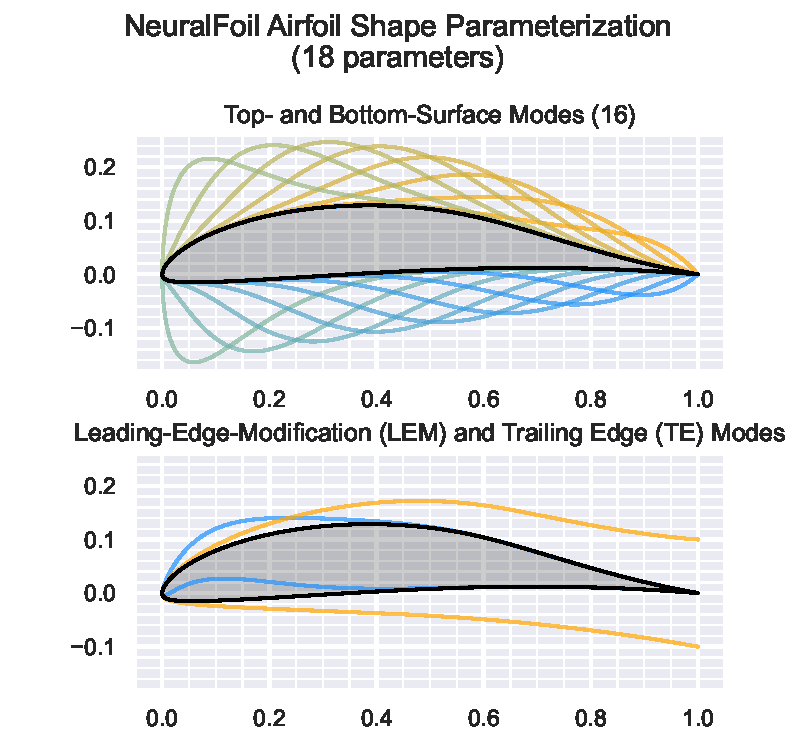
\includegraphics[width=0.8\textwidth]{../../media/kulfan_parameterization_illustration.pdf}
        \caption{Geometry input parameterization used by NeuralFoil.}
        \label{fig:neuralfoil_parameterization}
    \end{figure}

    Conversion of user-specified airfoils to this format for NeuralFoil to use is efficiently handled using the AeroSandbox framework, which formulates this as a least-squares fitting problem.

    \subsection{Model Architecture}

    NeuralFoil offers eight different deep neural network models, which offer a tradeoff between accuracy and computational cost. This tradeoff is implemented as differences in the number and size of hidden layers. Table \ref{tab:model-sizes} lists the different models, along with their number of hidden layers and neurons per hidden layer.

    \begin{table}
        \centering
        \caption{Neural network models offered in NeuralFoil.}
        \label{tab:model-sizes}
        \begin{tabular}{lll}
            \toprule
            Model        & Hidden Layers & Neurons per Hidden Layer \\ \midrule
            ``xxsmall''  & 2             & 32                       \\
            ``xsmall''   & 3             & 32                       \\
            ``small''    & 3             & 48                       \\
            ``medium''   & 4             & 64                       \\
            ``large''    & 4             & 128                      \\
            ``xlarge''   & 4             & 256                      \\
            ``xxlarge''  & 5             & 256                      \\
            ``xxxlarge'' & 5             & 512                      \\
            \bottomrule
        \end{tabular}
    \end{table}

    Each layer is a fully-connected linear layer. The activation function applied between each layer is a hyperbolic tangent function, which is chosen because the resulting model is $C^\infty$-continuous.

    \subsection{Training Data Generation}

    Training data was generated by

    \subsection{Training Process}

    \subsubsection{Loss Function}

    % TODO asymmetric CD penalty

    \subsection{Performance}

    XFoil


    \section{Reproducibility Statement}

    All code and data used in this paper is publicly available at \url{https://github.com/peterdsharpe/neuralfoil}. NeuralFoil itself is best accessed through the AeroSandbox \cite{sharpe_aerosandbox_2021} package, which provides some of the advanced features (e.g., $360\degree$ angle of attack, transonic effects, and control surface deflections) that are not yet available in the standalone NeuralFoil package.


    \section{Conclusion}
    \label{sec:conclusion}

    \section*{Acknowledgments}
    The authors acknowledge the MIT SuperCloud and Lincoln Laboratory Supercomputing Center for providing high-performance computing resources that have contributed to the research results reported within this work.

    \bibliography{main, C:/Users/peter/Documents/Zotero/library, C:/Users/peter/Documents/Zotero/library-zotero}

\end{document}
